\documentclass{standalone}
\usepackage{tikz}
\begin{document}
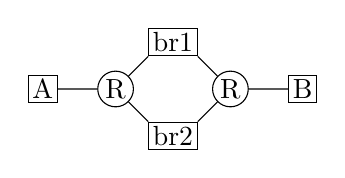
\begin{tikzpicture}
    \draw 
    node[rectangle, draw, inner sep=1.5pt](a)at(0,0){A}
    (a.0)--++(0.5,0)node[circle, draw, inner sep=1pt, anchor=west](r1){R}
    (r1.315)--++(0.25,-0.25)node[rectangle, draw, inner sep=1.5pt, anchor=north west](br2){br2}
    (r1.45)--++(0.25,+0.25)node[rectangle, draw, inner sep=1.5pt, anchor=south west](br1){br1}
    (br1.south east)--++(0.25,-0.25)node[draw, circle, inner sep=1pt, anchor=north west](r2){R}
    (br2.north east)--(r2.225)
    (r2.0)--++(0.5,0)node[draw, rectangle, inner sep=1.5pt, anchor=west](b){B}
    ;
\end{tikzpicture}
\end{document}